%!TEX root = ./report.tex
\section{Solution}
The provided solution consumes a set of 2D points  $P$ and returns  $D$ for performing point location queries in a Voronoi diagram corresponding to $P$. The attached CD contains the implementation as C\# source code that builds against .NET 4.0. An example providing $P$ and querying $D$ can be found in the program main.  A parser and example for generating data points from  the geographical coordinates of a set of fast-food restaurants is included. 
\paragraph{}
The solution is based on the description provided in \cite{computational_geometry} on point location and Voronoi diagrams, and as such, we do not cover the everything in detail, but rather provide highligts of parts that we found to be tricky to get right.  The implementation of Fortunes algorithm is an open-source implementation that can be found at [cite to misc and codeplex project] . Also , the solution includes a simple GUI from [cise to misc and ref to other os project] that can be useed to visualize simple small-scale datasets.  The implementation of $T$ and $D$ is provided by the authors and our main work constitues in implementing these, besides briding with Fortunes algorithm.
\paragraph{}
One way of accomplishing what we want would be to simply take to the output of Fortunes algorithm, that is, the generated edges, and give them as input to the algorithm for the trapezoidal map. Both algorithms run in O(nlogn)  so the the complexity of running the two in sequence is the same. Alternatively we could add the edges to $T$ on the fly as the are found by Fortunes. It is easy to see that we will get the same complexity as we are virtually doing the same thing. To show this easy connecting of the two algorithms, the implementation demonstrates the latter.

\subsection{Point location in Voronoi}
$D$ is implemented with a standard composite-pattern, and offers a $Find(point)$ operation that will return a bounding trapezoid for the query point.  Recall that a trapezoid is simply defined by its side points and top and bottom segment. And as each segment is just a segment w egot from the Voronoi diagram, it holds a reference to the site of the voronoi cell. Fortunes algorithm adds this edge to site reference, and, eventually, it is the only way that trapezoid can tell which Voronoi cells it lies in. Of course, queies will only be precise when all segments have been added, and all trapezoids are completely trapped inside Voronoi cells.
\paragraph{}
Each time a segment is discovered for the Voronoi diagram, it is inserted into the trapezoidal map, and $T$ is updated with new subtrees according to the new trapezoids that appear from the inserting the new segment. A this point a lot or re-wiring occurs, as new and existing trapezoids need to have their neighbourhoods re-wired correctly. One case of this is as seen in Figure~\ref{fig:contained_segment}. 

\begin{figure}[t]
    \centering
      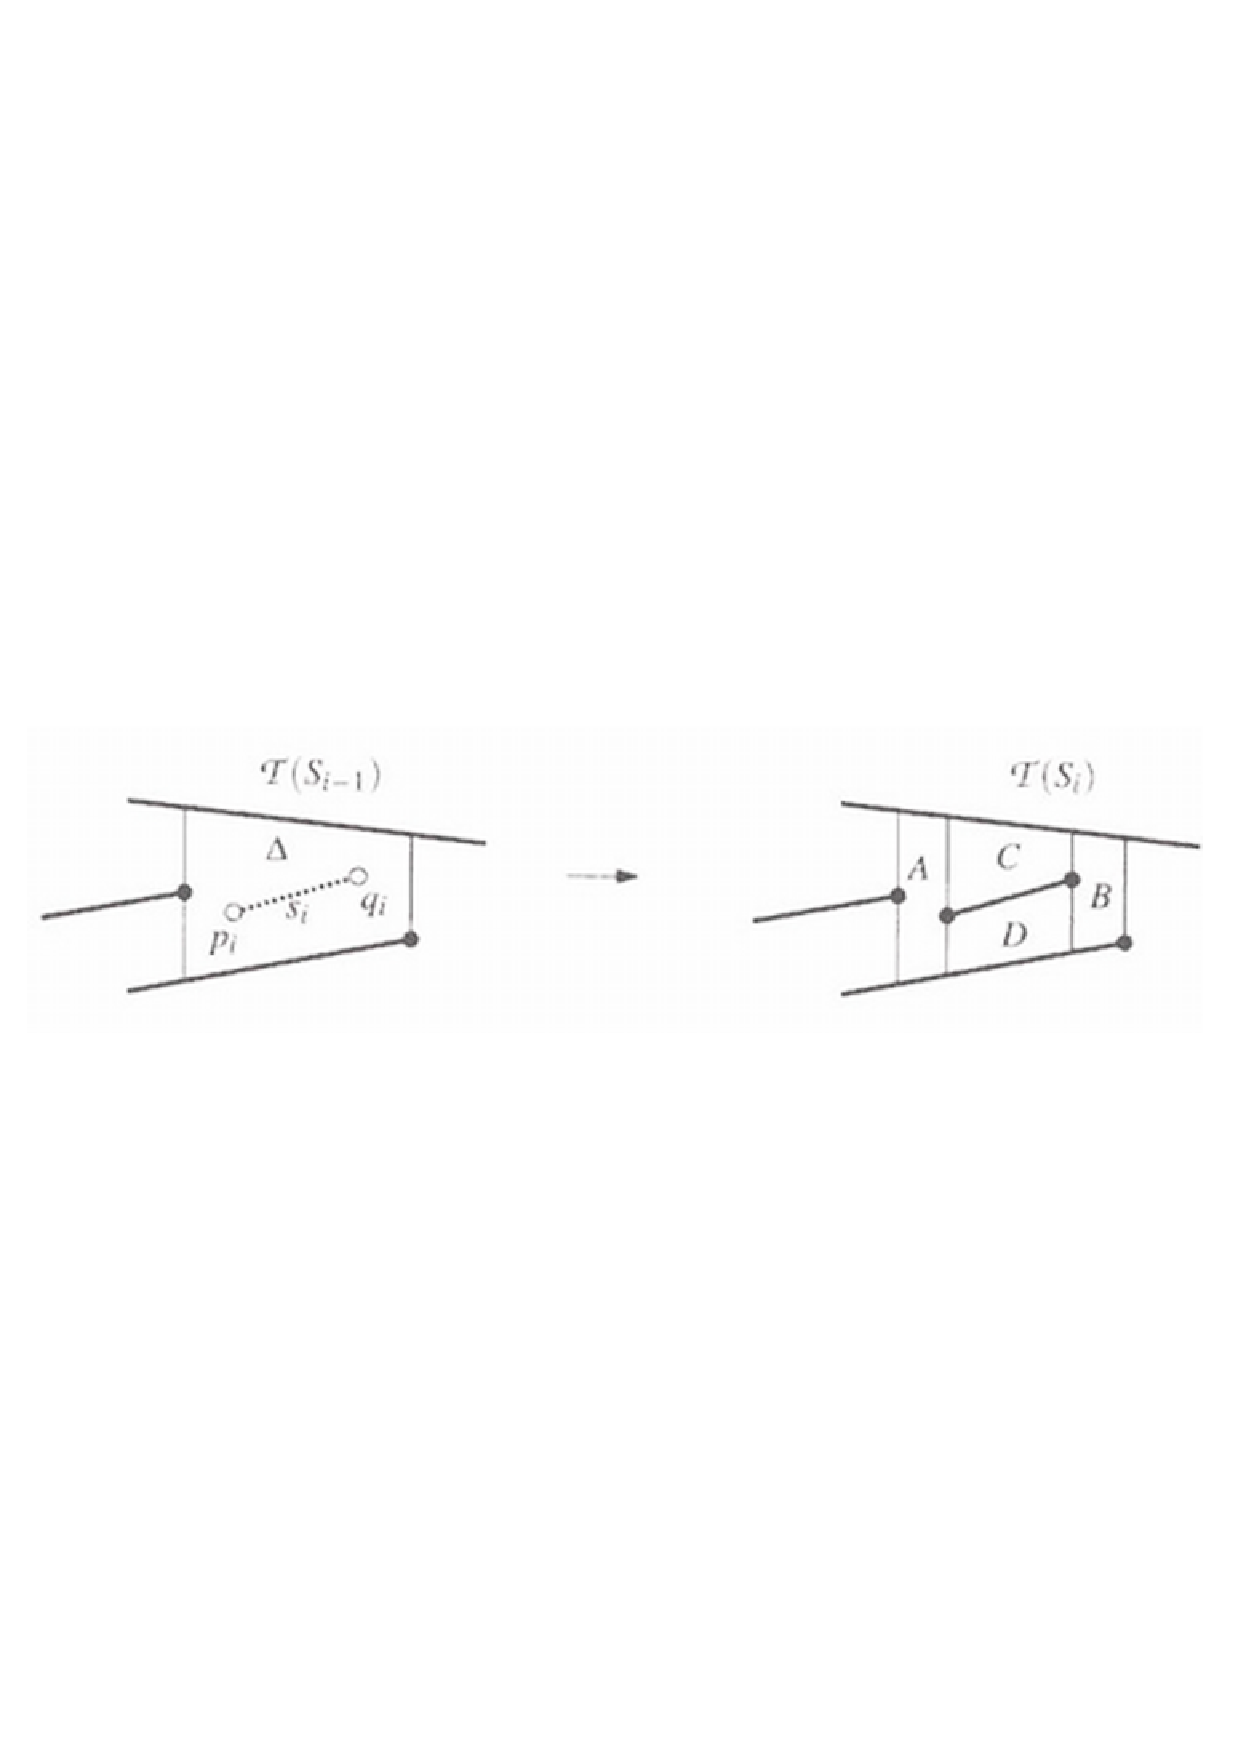
\includegraphics[height=80mm]{images/contained_segment.pdf}
    \caption{Inserting a segment in $T$ that is contained inside a single existing trapezoids}
    \label{fig:contained_segment}
\end{figure}

When the segment is contained in an existing trapezoid where we just need to make sure that we indetify what new trapezoids are created from inserting the segment, and updating $D$ with a corresponding subtree, which is somewat trival. In the case where a new segment crosses several existing trapezoids, things get a bit more tricky, and we will in the following explain how it can be solved.. The situation is depicted in Figure~\ref{fig:intersecting_segments}.\paragraph{}

\begin{figure}[t]
    \centering
      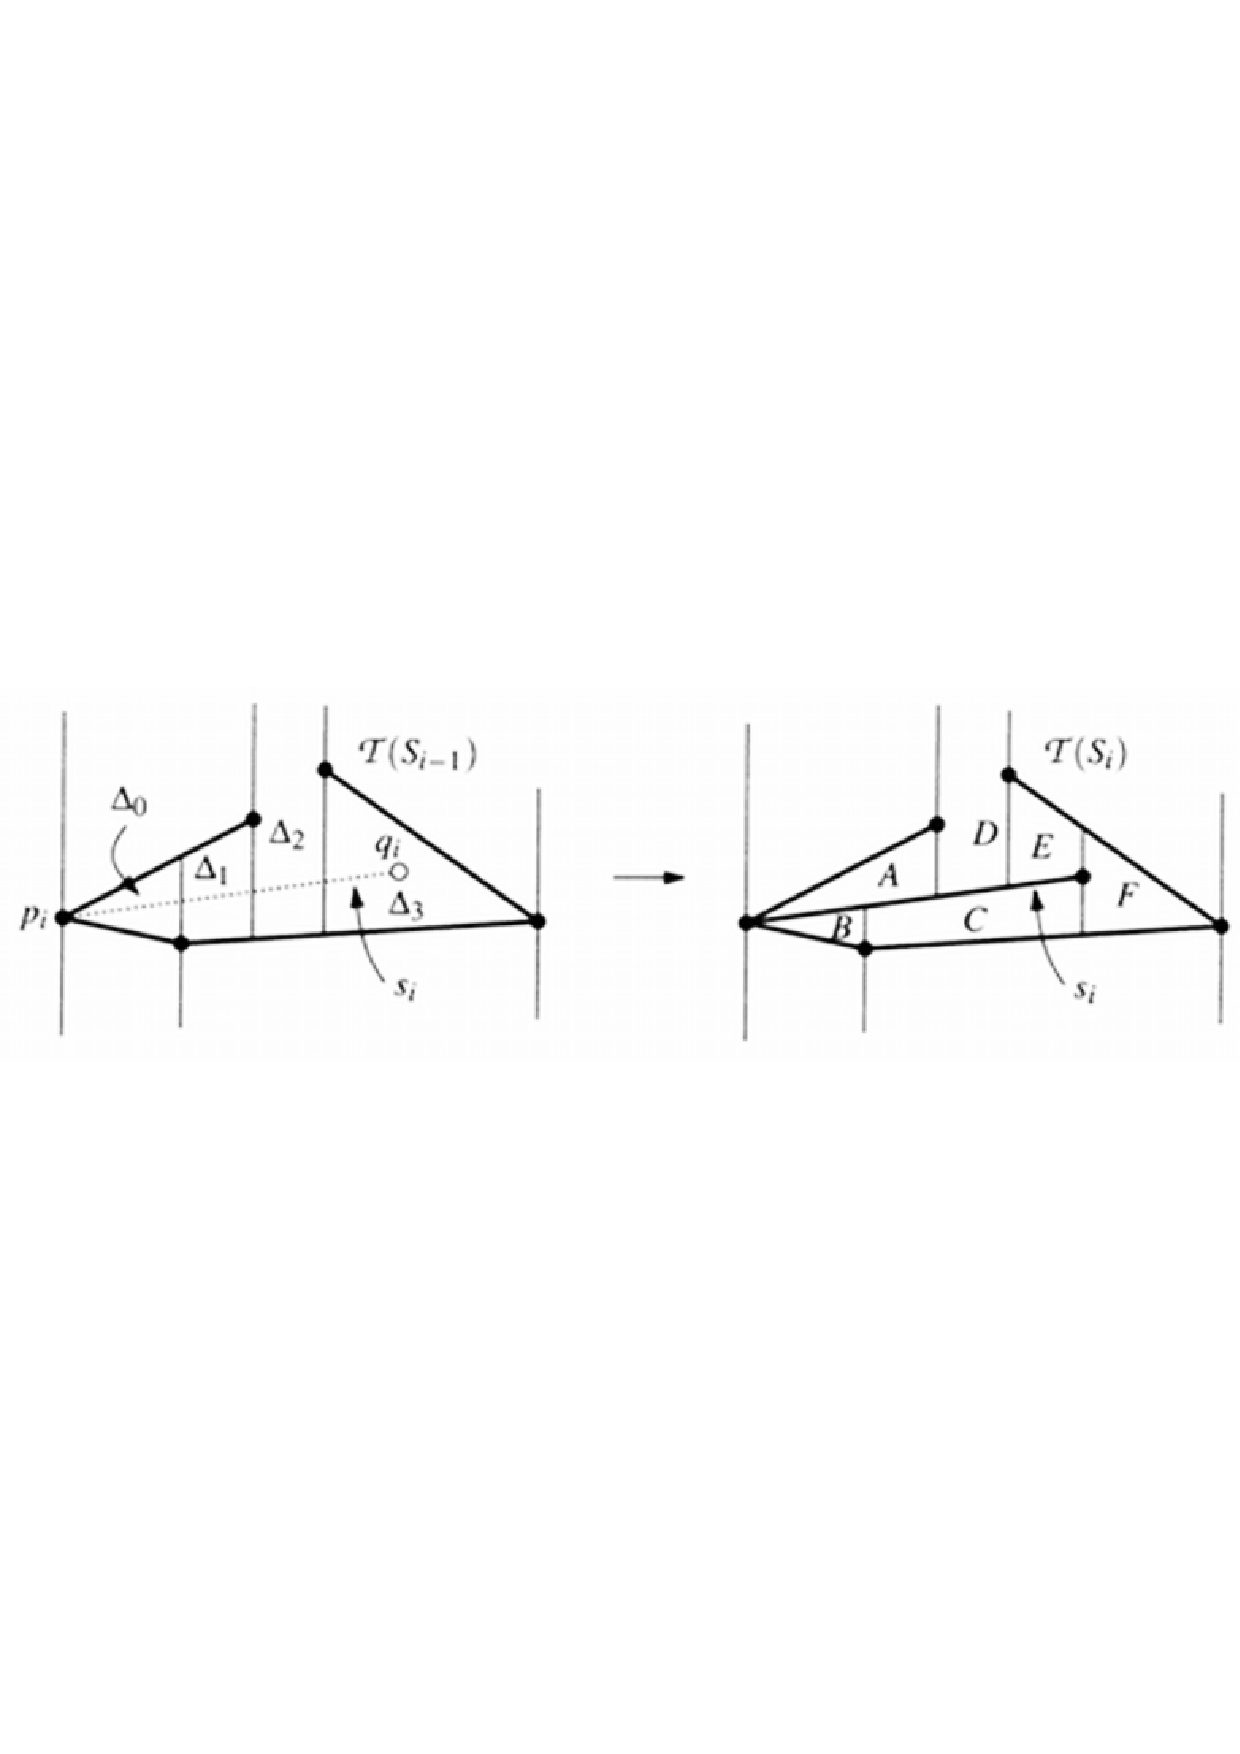
\includegraphics[height=80mm]{images/intersecting_segments.pdf}
    \caption{Inserting a segment in $T$ that crosses several trapezoids}
    \label{fig:intersecting_segments}
\end{figure}

\cite{computational_geometry} provides an good high-level description of how to handle this situation and states that it is done in linear time, which is possible as we can find neighbouring trapezoids by jumping from one trapezoid to the next by neighbour references - we do not need to look up neighbouring trapezoids in $D$. Now to handle the different case of the position of the inserted segment, we can start out by taking care of the boundries when one or both of the new segment's endpoints are connected to existing vertices, which is handled much like the the contained case. Secondly, we have to create new trapezoids that are, in some sense, horizontial merges of existing trapezoids. As an example, in Figure~\ref{fig:intersecting_segments}, we create  trapezoid $C$ with a left point from $\Delta 1$, a right point that will be the right most vertex of the newly inserted segment left most vertex, top being the new segment, and bottom being the the segment shared by  $\Delta 1$,  $\Delta 2$ and  $\Delta 3$.  Our solution to this is to always handle $\Delta 0$ and $\Delta 3$ in isolation, that is, add trapezoids much like with the case of the contained segment, and set the neighbourhoods. Secondly we do a recursive merge of the new trapezoids above the inserted segment, and under the segment. The pseudo code for doing an upper merge is show in Algorithm~\ref{alg:MERGEUPPER}.


\IncMargin{1em}
\begin{algorithm}
\label{alg:MERGEUPPER}
\SetKwData{Left}{left}\SetKwData{This}{this}\SetKwData{Up}{up}
\SetKwFunction{Union}{Union}\SetKwFunction{FindCompress}{FindCompress}
\SetKwInOut{Input}{input}\SetKwInOut{Output}{output}
\Input{A trapezoid $start$, a Segment $segment$, and a point $leftPoint$}
\Output{A list of trapezoids}
 \emph{Define LLN, ULN, LRN, URN as Lower Left Neighbour, Upper Left Neighbour, Lower Right Neighbour, Upper Right Neighbour of a trapezoid respectivly}\;
\Begin{
Create new trapezoid $t$\;
$t.leftPoint$ $\leftarrow$ $leftPoint$\;
$t.top$ $\leftarrow$ $start.top$\;
$t.bottom$ $\leftarrow$ segment\;
\BlankLine
$cur$ $\leftarrow$ $start$\;
\nl\While{$cur.rightPoint$ is below $segment$ and $cur$ is on the $segment$}{
	$cur$ $\leftarrow$ cur.URN;
}
\BlankLine
\nl\If{$segment.RightMostVertex.X$ $<$ $cur.RightPoint.X$}{
		$t.RightPoint$  $\leftarrow$ segment.RightMostVertex\;
	\lElse{
		$t.RightPoint$  $\leftarrow$ $cur.RightPoint$\;
	}
}
\BlankLine
\nl\If{$cur.rightPoint$ is before end of segment}{
        next $\leftarrow$ $MergeUpper(cur.LRN, segment,  cur.rightPoint)$\;
        $t.LRN$  $\leftarrow$ $next.First$\;
        $t.URN$ $\leftarrow$ $cur.URN$\;
}
 \Return{$t$ and $next$}\;
}
\caption{MergeUpper}\label{algo_disjdecomp}
\end{algorithm}\DecMargin{1em}

Doing a merge of the trapezoids below the inserted segment is done the same way, but with the neighbouring reference flipped horizontially. The last thing we need to do is to update $D$. 

\IncMargin{1em}
\begin{algorithm}
\label{alg:INSERTMERGED}
\SetKwData{Left}{left}\SetKwData{This}{this}\SetKwData{Up}{up}
\SetKwFunction{Union}{Union}\SetKwFunction{FindCompress}{FindCompress}
\SetKwInOut{Input}{input}\SetKwInOut{Output}{output}
\Input{A list of existing trapezoids $olds$, a list of upper merged trapezoids $upper$, and a list of lower merged trapezoids $lower$, and the inserted $segment$}
\KwResult{Updated search tree $D$}
\Begin{
let $i$ $\leftarrow$ $j$ $\leftarrow$ $k$ $\leftarrow$ 0\;
\BlankLine
\nl\While{$k$ $\textless$ $olds.Count$}{
\BlankLine
	\nl\While{$upper[j].RightPoint.X$ $\textless$ $olds[k].RightPoint.X$}{
		$j$ $\leftarrow$ $j$ + 1\;
	}
\BlankLine
	\nl\While{$lower[i].RightPoint.X$ $\textless$ $olds[k].RightPoint.X$}{
		$i$ $\leftarrow$ $i$ + 1\;
	}
\BlankLine
	Replace $olds[k]$ with subtree of $segment$, $upper[j]$ and $lower[j]$ in $D$
\BlankLine
	$k$ $\leftarrow$ $k$ + 1\;
}
\BlankLine
}
\caption{InsertMergedTrapezoids}
\end{algorithm}\DecMargin{1em}

%Explain merge of cells situation, and maybe provide pseudo code of how we did it.
%Discuss implementaion dificulties, like updating neighbours, unprecise doubles in search tree.
%Porlbmees with voronoi implemenation, stuff that probably doesnt work with real fast food restaurant data set.

\subsection{Expected Customers}
%Expected number of hits by random shooting of points on the map. Chernoff expectation vs size of voron oi cells.

